\documentclass{TDP003mall}


\newcommand{\version}{Version 1.0}
\author{Adam Ivarsson, \url{adaiv505@student.liu.se}\\
  Lukas Michanek, \url{lukmi182@student.liu.se}}
\title{User Manual}
\date{2015-09-17}
\rhead{Adam Ivarsson\\
Lukas michanek\\}


\begin{document}
\projectpage


\section{User Manual}\label{user-manual}

This user manual will walk through the structure of the portfolio out and how to use it.


\section{Layout Structure}\label{layout-structure}

All pages inherit the base portfolio layout. This layout has a few elements that stay concistent throughout all pages:

\begin{itemize}
    \item The sidebar, which contains information \textbf{about} the webpage. The sidebar has:
    \begin{itemize}
        \item A picture of the portfolio owner.
        \item Short info about the owner.
        \item Navigation list with links to:
        \begin{itemize}
            \item The start page.
            \item The list page.
            \item The techniques page.
        \end{itemize}
    \end{itemize}
    \item The portfolio logo and title.
\end{itemize}


\section{Blog Structure}\label{blog-structure}

The front-end of your portfolio will consist of 4 pages (see list below):

\begin{itemize}
    \item The Startpage (\texttt{/})
    \item Contains a ``featured'' post.
    \item This page should look about the same as a project page.
    \item The List Page (\texttt{/list})
    \item Contains a list of all projects where each row consists of the following information:
      \begin{itemize}
          \item The project name.
          \item An image from the post.
          \item A short description.
      \end{itemize}
    \item Has search functionality for filtering by text and techniques (any or all of the selected) with functions for sorting (ascending or decending date).
    \item Clicking on the title of a post will bring you to the project page for that project.
    \item The Project Page (\texttt{/project/id})
    \item Presents all available information about a project to the user. This includes, but is not limited to:
      \begin{itemize}
          \item The project name.
          \item The project date (day, month, year).
          \item All involved parties (ex. team members).
          \item Techniques used, as a list of clickable tags. Clicking on one tag should bring you to the \texttt{/list} page, filtered by the tag you clicked on.
      \end{itemize}
    \item The Techniques Page (\texttt{/techniques})
    \item Contains a list of all techniques used throughout all projects, followed by a list of all project that use that certain technique.
    \item Clicking a project name will take you to that project's project page.
    \item Clicking a technique name will take you to the list page filtered by the technique you clicked.
\end{itemize}


\section{Searching and Filtering}\label{searching-and-filtering}

The list page contains a form to request projects matching your search and filtering criteria. Once requested the server will retrieve all matches, sort them, and then send them back to you. To do this you'd have to fill out the search and filtering form.

The form itself is divied up in two sections where the first section filters results based on selected techniques (checkboxes), and where the second section lets you select a sorting method and search projects by text. This is roughly what the form looks like:

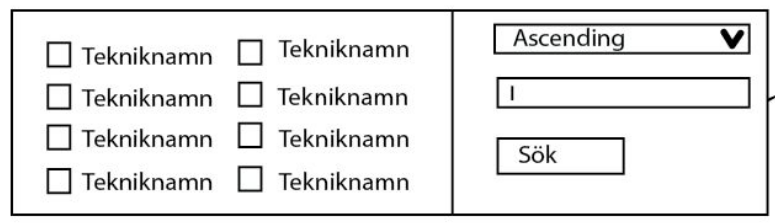
\includegraphics[width=\textwidth]{search_box}

These projects may then be sorted by date using the dropdown list and
choosing either \texttt{Ascending} or \texttt{Decending}.

Additionaly, there is a text search box if you'd rather prefer that.

\end{document}
